\chapter{Diseño detallado}
\label{cap:diseno-detallado}

En este capítulo se presenta el diseño detallado de la solución implementada en
el proyecto.  Se detalla el proceso de extracción, transformación y carga de
información.

\section{Dependencias y frecuencia de las extracciones de datos}

Como primer paso dentro del proceso de extracción se identificaron las
dependencias de los sistemas origen con otros procesos, tareas o reglas de
negocio dentro de la organización, así como la frecuencia esperada o deseada de
la extracción de datos. La extracción de datos se realizó con una periodicidad
diaria; esto debido a que al tratarse del sistema principal de la institución
financiera la información se actualizaba con esa periodicidad. La herramienta
ETL nos permitió identificar aquellas tablas y campos que sufrían
modificaciones, de tal forma que se extrajo sólo la información que sufría
cambios a lo largo del día. La extracción de datos se realizó en un horario no
operativo, a fin de no afectar la operación de la institución; además este
proceso dependía del termino del proceso de cierre diario de
operaciones. Solamente una vez que el proceso hubiera terminado comenzaba la
extracción por parte de la herramienta ETL; este proceso contaba con una ventana
de procesamiento de 5 horas. La extracción fue almacenada en la base de datos
temporal dentro de la herramienta ETL.

\subsection{Extracción inicial}

En la extracción inicial se realizaron las siguientes transformaciones:

\begin{itemize}
\item Transformación de fecha juliana a fecha gregoriana.
\item Cambio en los tipos de datos al momento de almacenarlos en la tabla
  temporal; principalmente transformación del tipo de dato \textit{char} al tipo
  de dato \textit{varchar} y los datos numéricos a decimal.
\end{itemize}

Al momento de que se terminaba la extracción de datos, se cerraba la conexión a
la base de datos del procesador principal de transacciones bancarias a fin de
liberar la carga de trabajo del mismo para continuar con su operación diaria.

\subsection{Extracciones subsecuentes}

Después de realizada la extracción inicial desde el sistema fuente y con los
datos almacenados en el repositorio temporal, las siguientes extracciones se
realizaron mediante extracciones incrementales con base en la adición,
actualización o eliminación de datos de las tablas seleccionadas. Se consideró
realizar la extracción total de los registros sólo en caso de que las
modificaciones o actualizaciones en la base de datos fueran muchas; las
condiciones para realizar la extracción completa fueron las siguientes:

\begin{enumerate}
\item Existían cambios en más del 50\% de los registros.
\item Los registros extraídos no se encontraban actualizados o contenían
  errores.
\item Los registros extraídos no cuentan con la calidad necesaria.
\end{enumerate}

\subsection{Relación entre las entidades de datos}

En la figura~\ref{fig:datos-relacionados-en-las-entidades} se puede visualizar
la relación entre las diferentes entidades y los datos que comparten cada uno de
ellos.

\begin{figure}[htb]
  \begin{center}
    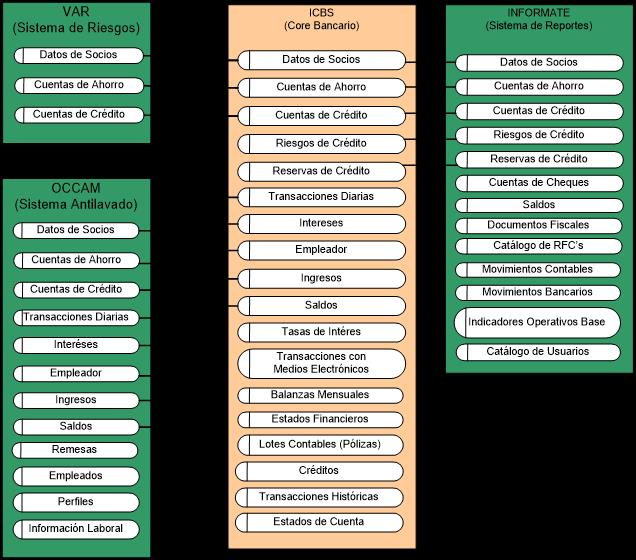
\includegraphics[width=\linewidth]{Relacion_entidades.jpg}
        \caption{Datos relacionados en las entidades.}
    \label{fig:datos-relacionados-en-las-entidades}
  \end{center}
\end{figure}

En la misma podemos observar que los diferentes sistemas manejan el mismo tipo
de información; socios, cuentas, créditos y saldos.

\section{Diseño para la transformación de datos}

La transformación de los datos tenía varios procesos que se deberían seguir,
entre los cuales se encontraba la limpieza de datos, los estándares y
procedimientos utilizados, así como las reglas de transformación definidas para
cada uno de los sistemas destino. La transformación de los datos se realizó
dentro de la misma base de datos de paso y se almacenó en otra instancia de esta
misma base de datos. La
figura~\ref{fig:transformaciones-en-base-de-datos-temporal} muestra cómo se
realizaron las transformaciones requeridas.

\begin{figure}[htb]
  \begin{center}
    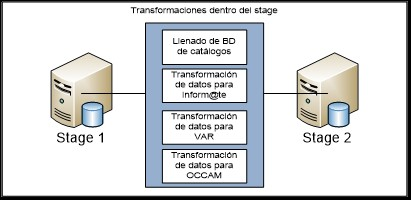
\includegraphics[width=0.7\linewidth]{Transformaciones_stage.jpg}
    \caption{Transformaciones en base de datos temporal.}
    \label{fig:transformaciones-en-base-de-datos-temporal}
  \end{center}
\end{figure}

A continuación se detallan las reglas utilizadas para realizar la transformación
de datos.

\subsection{Limpieza de la fuente de datos}

La limpieza de la fuente de datos \textbf{NO} estaba dentro del alcance del
proyecto; sin embargo se realizaron las transformaciones de la fuente de datos
para realizar la limpieza de datos hacia los sistemas destino. Como parte de un
proceso de calidad de la información y limpieza de datos se definieron los
siguientes criterios:

\begin{enumerate}

\item Los nombres de los socios debían contener solamente caracteres
  alfabéticos; no se permitieron caracteres especiales como los siguientes:
  ``\textbackslash'', ``.'', ``\#'', ``\$'', ``\%'', ``\&''.

\item Los números telefónicos debían contener solamente caracteres numéricos y
  debían ser de 10 posisciones para teléfonos fijos y 13 posiciones para
  teléfonos celulares.

  \begin{itemize}
  \item Si \textit{Tipo\_Telefono} $=$ Casa y Longitud $($Telefono$)$ $=$10
    Entonces Telefono\_Casa SiNo Error
  \item Si \textit{Celular} $=$ Casa y Longitud $($Telefono$)$ $=$ 13 Entonces
    Telefono\_Celular SiNo Error
  \end{itemize}

\item El RFC de los socios debería ser de 10 o 13 posiciones para las personas
  físicas y 12 posiciones para las personas morales. En caso de no contar con un
  RFC valido, el registro era rechazado y enviado a una tabla de auditoría para
  su corrección dentro del sistema fuente de parte del área de tecnología de la
  compañía.

\item Todos los códigos postales debían ser de cinco dígitos, en caso de existir
  algún registro con mayor o menor número, estos debían de ser enviados a una
  tabla de auditoría para su corrección dentro del sistema fuente. Se consideró
  una homologación de datos para los códigos de ciudades y estados. Todos los
  códigos de estados se homologaron a tres dígitos que corresponden a las tres
  primeras letras de cada estado; se realizó una excepción para el caso de
  Chiapas (CHS) que podría confundirse con Chihuahua (CHI).

\item Las fechas se homologaron al formato yyyymmdd y no debían permitir valores
  nulos o fechas inválidas.

\end{enumerate}

\subsection{Estándares y procedimientos utilizados para la interrelación de los datos}

Para realizar una estandarización de los datos se creó una base de datos
temporal que contenía la información de todos los campos con los mismos datos
pero que su sistema origen era diferente. La creación de esta tabla temporal fue
crear la base para generar una tabla de referencias cruzadas que representara un
gobierno de datos o MDM (\emph{Master Data Management}) por sus siglas en
inglés.

\subsection{Reglas utilizadas para la transformación de datos}

Como regla general para todos los procesos de extracción se realizaron las
siguientes transformaciones.

\begin{itemize}
\item Transformación de fechas julianas a fechas gregorianas en formato
  \linebreak \mbox{yyyy/mm/dd}.
\item Transformación de los tipos de dato origen a los tipos de la base de
  datos \emph{stage} generada en SQL Server.
\end{itemize}

Los procesos de transformación para cada destino fueron diferentes debido a las
características de cada uno de los archivos de salida. Dichas transformaciones
se realizaron tomando como principal fuente de datos la base de datos temporal.

\subsubsection{Sistema de reportes}

\begin{itemize}

\item Todos los campos de fecha que tengan un sufijo \_d deberían de ser
  convertidas a formato de fecha $($yyyymmdd$)$ para todas las tablas de este
  sistema. Se pobló la fecha de vencimiento \_D, tomando como base el campo
  fecha de vencimiento de la tabla de facturación. La regla de transformación
  que se definió fue la siguiente:

{\footnotesize
\begin{verbatim}
FEC_VENCIMIENTO_5_D = CAST(
  RIGHT(
    LTRIM(
      RTRIM(
        FEC_VENCIMIENTO_5)
      ), 2
    ) +
    LEFT(
      RIGHT(
        LTRIM(
          RTRIM(
            FEC_VENCIMIENTO_5
          )
        ), 4
      ), 2
    ) +
    REPLICATE(
      '0', 2 - (
        LEFT(
          LTRIM(
            RTRIM(
              FEC_VENCIMIENTO_5
            )
          ),
          ABS(
            4 - len(
              LTRIM(
                RTRIM(
                  FEC_VENCIMIENTO_5
                )
              )
            )
          )
        )
      )
    ) +
    LEFT(
      LTRIM(
        RTRIM(
          FEC_VENCIMIENTO_5
        )
      ),
      ABS(
        4 - len(
          LTRIM(
            RTRIM(
              FEC_VENCIMIENTO_5
            )
          )
        )
      )
    ) AS DATETIME
  ) WHERE FEC_VENCIMIENTO_5 > 0
\end{verbatim}
}

\item Para el campo de fecha de último saldo se tomó la fecha de vencimiento más
  antigua que se tenía.
\item Para obtener el número de créditos de un socio se realizó la siguiente
  regla.

\begin{verbatim}
  NO_CREDITOS =  NO_CREDITOS
    WHERE NO_SOCIO IN NO_SOCIO de la tabla CIF_CREDITOS.
  Si NO_CREDITOS = NULL Entonces NO_CREDITOS = 0
\end{verbatim}

\item La descripción de la información correspondiente a las garantías debía
  de estar vacía en la tabla destino.

\item Para almacenar la fecha de último monto con saldo se tomó la fecha de
  vencimiento más antigua que se tenía para cada registro dentro de la tabla de
  saldos LN\_SALDOS.

\item Se realizó una validación sobre el tipo de cuenta para confirmar su valor
  igual a 1 (Personas físicas) o 6; en estos casos se colocó un valor 20 dentro
  del campo Tipo\_producto de la tabla TA\_SALDOS.

\item El número de socio para poblar la tabla TA\_SALDOS se obtuvo de la
  tabla de cuentas por socio, pero solamente de aquellas cuentas cuyo tipo de
  producto era 4 u 8 y que tuvieran un saldo en la tabla TA\_SALDOS.

\item Se calculó el número de créditos de cada socio y este valor se grabó en
  la tabla CIF\_INFGEN; en caso de que el número de créditos fuera nulo se
  colocó un valor por omisión cero.

\item Se insertó el número de socio dentro de la tabla TA\_CTAXSOCIO para
  aquellos números de cuenta menores a 20000000000 y cuya clave de relación
  fuera `SOW' u `OWN'. El número de socio eran los 10 dígitos de la derecha de
  cada número de cuenta.

\item Se definió que para el campo descripción perteneciente a la tabla
  LN\_GARANTIAS debería poblarse con un valor NULL a pesar de tener mapeado un
  campo del cuál se extraía la información.

\item El campo Periodo de la tabla LN\_SALDOS se asignó con un valor fijo =
  `M'.

\item El campo frecuencia de la tabla LN\_SALDOS se asignó con un valor fijo
  $=$ 30.

\end{itemize}

La regla de transformación que se utilizó durante la extracción.
% Esto no compila.

\subsubsection{Reglas para el sistema para prevención de lavado de dinero}

Las reglas definidas para este sistema son las siguientes:

\begin{itemize}
\item Se definieron algunos valores estáticos para los tres primeros campos de
  cada uno de los archivos generados; estos valores son los siguientes:
\begin{enumerate}
\item Valor fijo `CMPS' para el primer campo.
\item Valor fijo `T' para el segundo campo.
\item Valor fijo `F' para el tercer campo.
\end{enumerate}
\item Para la generación del archivo de cuentas se tomaron sólo aquellas
  cuentas que tuvieron movimientos durante el día.
\item Solamente se tomaron en cuenta los siguientes tipos de cuenta: Parte
  social, cuenta mexicana, servicuenta y cuentamiga.
\item Si el tipo CIF es una persona moral (CUTYP $=$ 5), entonces el campo
  CompanyLegalId se pobló con dicho valor, en caso contrario se asignó un valor
  constante vacío ``''.
\end{itemize}

\section{Arquitectura aplicativa}

La arquitectura aplicativa requerida para un proceso de extracción,
transformación y carga de datos está comprendida por una herramienta ETL y
algunos componentes de software adicionales para lograr la integración de la
solución.

El modelos de aplicaciones por lotes (\emph{batch}) que se muestra a
continuación ilustrará los componentes de la arquitectura que fueron requeridos
para la implementación del proyecto. Este modelo fue desarrollado con base en
las mejores prácticas para el uso de aplicaciones por lotes de tipo ETL.

\subsection{Capas de la arquitectura}

El esquema de las aplicaciones tipo por lotes incluye los servicios necesarios para
apoyar los procesos que se ejecutan durante largos periodos de tiempo y que
ejecutan tareas de manera repetitiva. En este esquema de aplicación, un programa
generalmente lee un número grande de registros de una base de datos o de un
archivo, procesa los datos y luego escribe datos transformados a una base de
datos o a un archivo.

Del marco de trabajo (\emph{framework}) de aplicaciones por lotes encontramos
las siguientes capas principales:

\begin{itemize}
\item Ejecución.
\item Proceso por lotes.
\item Aplicaciones por lotes.
\item Negocios.
\item Datos.
\end{itemize}

El marco de trabajo comprende componentes que brindan servicios a las capas
principales de la cuales son:

\begin{itemize}
\item Servidores de aplicación.
\item Flujos de trabajo de usuarios.
\item Captura de datos.
\item Servicios por lotes.
\item Servicios de reportes.
\item Servicios de gestión.
\item Servicios de seguridad.
\item Servicios comunes.
\end{itemize}

En las siguientes secciones se describirá la responsabilidad de cada una de las
capas.

\subsection{Componentes de la capa de presentación}

Dentro de la capa de presentación se tienen varios componentes entre ellos el
panel de consulta y la interfaz de usuario que nos ayuda a la revisión y
monitoreo del proceso por lotes; así como los resultados que éste arroja.

\subsection{Servicios de la capa de presentación}

Los servicios que brindan los componentes de esta capa de a acuerdo al marco de
trabajo utilizado son los siguientes:

\begin{enumerate}
\item Monitoreo de programa.
\item Reportes.
\item Servicios comunes.
\end{enumerate}

\subsubsection{Monitoreo de programas}

Este servicio proporciona las herramientas para monitorear cuáles programas y
aplicaciones están siendo ejecutados, así como la información a nivel sistema
del uso de recursos. El monitoreo de programas puede actuar como entrada
principal en las decisiones de balanceo de cargas.

\subsubsection{Reportes}

Reportes permiten al usuario dar formato a los resultados de una consulta dentro
de la producción de reportes de calidad.

\subsection{Componentes de la capa de ejecución}

Los componentes encontrados en esta capa de acuerdo al marco utilizado son los
siguientes:

\begin{itemize}
\item Calendarizador de tareas (\emph{scheduler}).
\item \emph{Script} de ejecución de programas.
\item Proceso por lotes.
\end{itemize}

Los componentes de esta capa son los encargados de comenzar con el proceso de
ejecución y se describen a continuación:

\subsubsection{Calendarizador}

El servicio de calendarización proporciona la estructura de control para
programas por lotes; esto es, administra el flujo de su procesamiento. Un
proceso de calendarización debe de proporcionar una interfaz de usuario para
entrar y dar mantenimiento a la información y a la calendarización de los
procesos por lotes.

\subsubsection{\emph{Scripts} de ejecución de programas}

Este servicio es responsable de establecer y restaurar el ambiente en el cuál el
proceso por lotes es ejecutado; también debe ser capaz de ser ejecutado por el
calendarizador así como recibir y/o enviar parámetros del calendarizador al
proceso por lotes, tales como el nombre del proceso a ser ejecutado. El
\emph{script} debe proporcionar los procedimientos y guía necesarios para
ejecutar el proceso por lotes.

\subsubsection{Proceso por lotes}

Un proceso por lotes controla la ejecución de la aplicación. Un proceso por
lotes es típicamente un script de ejecución que control el orden del proceso,
nombres de archivos de entradas/salidas y dependencias entre procesos por lotes.

\subsection{Servicios de la capa de trabajos programados (\emph{Jobs})}

Los servicios que soportan a los componentes de esta capa de acuerdo al
framework utilizado son los siguientes:

\begin{itemize}
\item Reinicio / Recuperación.
\item Trabajos particionados.
\item Servicios comunes
\end{itemize}

\subsubsection{Reinicio y recuperación}

El servicio de reinicio y recuperación permite a los proceso programados
apagarse y reiniciarse en puntos apropiados después de una interrupción anormal
o de la intervención del usuario.

\subsubsection{Trabajos particionados}

Usando una partición, permite que múltiples versiones de aplicaciones
programadas se ejecuten concurrentemente. El propósito de esto es reducir el
tiempo transcurrido que se requiere para procesar la información.

\section{Arquitectura de negocio}

Esta capa se divide en 4 grandes módulos que contienen toda la lógica de negocio
los cuales son:

\begin{enumerate}
\item Extracción
\item Limpieza.
\item Transformación.
\item Carga
\end{enumerate}

\subsection{Módulo de extracción}

Extracción es el proceso que consiste de los módulos que extraen los datos de
una fuente(s) de datos determinada.  El módulo de extracción está formado de los
siguientes componentes.

\begin{enumerate}
\item Monitor de tareas programadas.
\item Monitor de \textit{Triggers}
\item Adaptadores de fuente de datos.
\item Filtrado y búsqueda de datos.
\item Estandarización de tipos de tato

\end{enumerate}

\section{Arquitectura de datos}

Como se explicó en los capítulos anteriores, la institución financiera contaba
con diferentes procesos ETL que extraían información del sistema
principal. Estos sistemas trabajaban de manera independiente por lo que cada
sistema destino tenía su base de datos temporal antes de enviarla a su
destino. La arquitectura se encuentra detallada en la
figura~\ref{fig:arquitectura-de-datos-actual}.

\begin{figure}[htb]
  \begin{center}
    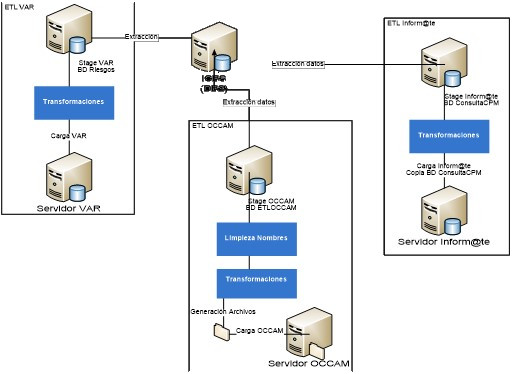
\includegraphics[width=0.8\linewidth]{Arquitecturadatos_actual.jpg}
    \caption{Arquitectura de datos actual.}
    \label{fig:arquitectura-de-datos-actual}
  \end{center}
\end{figure}

Como se observa en la figura~\ref{fig:arquitectura-de-datos-actual}, existían
muchas bases de datos intermedias entre la fuente de datos y los sistemas
destino; la arquitectura definida dentro de este proyecto, nos permite tener una
sola base de datos temporal, así como una sola capa de integración de datos. El
siguiente diagrama muestra el diseño de la arquitectura desarrollada:

\begin{figure}[htb]
  \begin{center}
    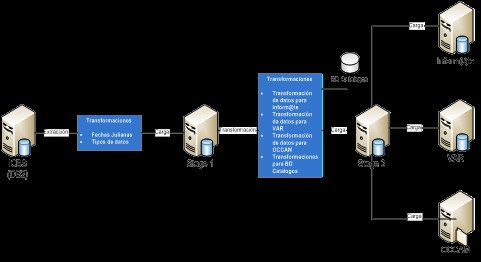
\includegraphics[width=0.8\linewidth]{Arquitectura_final.jpg}
    \caption{Arquitectura de datos final.}
    \label{fig:arquitectura-de-datos-final}
  \end{center}
\end{figure}

Arquitectura\_final % ???

\section{Arquitectura de infraestructura}
Como parte de la solución propuesta se describirá la infraestructura con la cuál la institución financiera debe de tener en los diferentes ambientes para la implementación de la solución ETL.
A lo largo del capítulo se especifican los componentes de hardware y software necesario. 

\subsection{Ambiente de producción}
Se describe a continuación las especificaciones de los servidores físicos requeridos.

\begin{table}[htbp]
  \begin{center}
    \begin{tabular}{|p{6cm}|>{\centering\arraybackslash}m{3cm}|c|}
      \hline
      Modelo & Servidor & Sistema Operativo &  Aplicaciones / Programas & Tipo base de datos\\
      \hline
      iSeries & ICBS PRO & OS / 400 &  & DB2 \\
      \hline
      Dell tipo rack & Informate PRO DB & Windows 2003 estándard & Configuration Manager SQL, aplicaciones web, reportes & \\
      \hline
      Dell tipo rack & Informate PRO DB & Windows 2003 estándard & Oracle DB2, SQL Server 2005 & SQL 2005\\
      \hline
      HP Proliant BL 460c G1 Tipo Blade & OCCAMPRO & Windows 2003 estándar & Visual estudio 2005, SQL server 2005, Apache tomcat, office 2003 & SQL 2005.\\
      \hline
    \end{tabular}
    \caption{Infraestructura requerida.}
    \label{tab:infraestructura requerida}
 \end{center}
\end{table}

El diagrama de red de la infraestructura mencionada se muestra a continuación

\begin{figure}[htb]
  \begin{center}
    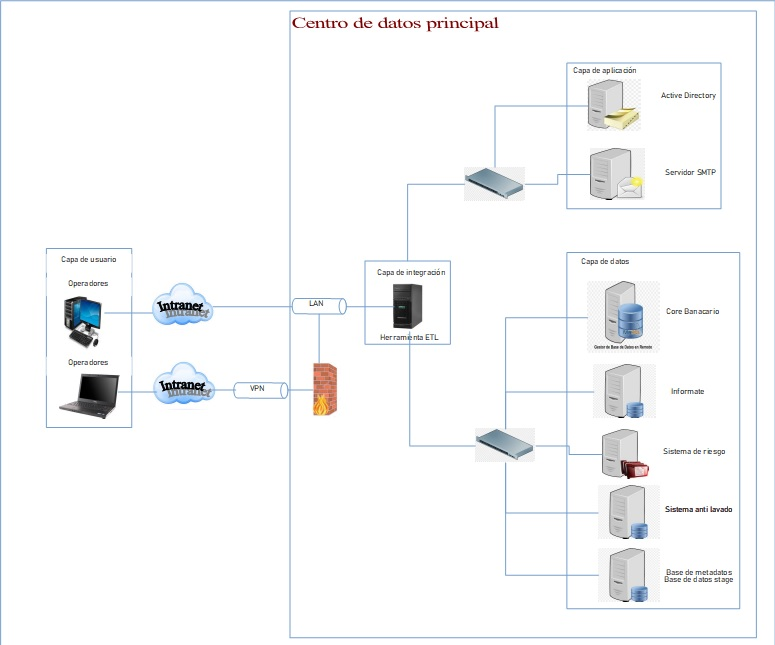
\includegraphics[width=0.8\linewidth]{Infraestructura.jpg}
    \caption{Infraestructura de aplicación.}
    \label{fig:infraestructura}
  \end{center}
\end{figure}   

\cleardoublepage

%%% Local Variables:
%%% TeX-master: "Tesis"
%%% End:
